\documentclass[11pt,a4paper,]{article}
\usepackage{lmodern}

\usepackage{amssymb,amsmath}
\usepackage{ifxetex,ifluatex}
\usepackage{fixltx2e} % provides \textsubscript
\ifnum 0\ifxetex 1\fi\ifluatex 1\fi=0 % if pdftex
  \usepackage[T1]{fontenc}
  \usepackage[utf8]{inputenc}
\else % if luatex or xelatex
  \usepackage{unicode-math}
  \defaultfontfeatures{Ligatures=TeX,Scale=MatchLowercase}
\fi
% use upquote if available, for straight quotes in verbatim environments
\IfFileExists{upquote.sty}{\usepackage{upquote}}{}
% use microtype if available
\IfFileExists{microtype.sty}{%
\usepackage[]{microtype}
\UseMicrotypeSet[protrusion]{basicmath} % disable protrusion for tt fonts
}{}
\PassOptionsToPackage{hyphens}{url} % url is loaded by hyperref
\usepackage[unicode=true]{hyperref}
\hypersetup{
            pdftitle={Immigration Report},
            pdfborder={0 0 0},
            breaklinks=true}
\urlstyle{same}  % don't use monospace font for urls
\usepackage{geometry}
\geometry{a4paper, centering, text={16cm,24cm}}
\usepackage[style=authoryear-comp,]{biblatex}
\addbibresource{references.bib}
\usepackage{longtable,booktabs}
% Fix footnotes in tables (requires footnote package)
\IfFileExists{footnote.sty}{\usepackage{footnote}\makesavenoteenv{long table}}{}
\usepackage{graphicx,grffile}
\makeatletter
\def\maxwidth{\ifdim\Gin@nat@width>\linewidth\linewidth\else\Gin@nat@width\fi}
\def\maxheight{\ifdim\Gin@nat@height>\textheight\textheight\else\Gin@nat@height\fi}
\makeatother
% Scale images if necessary, so that they will not overflow the page
% margins by default, and it is still possible to overwrite the defaults
% using explicit options in \includegraphics[width, height, ...]{}
\setkeys{Gin}{width=\maxwidth,height=\maxheight,keepaspectratio}
\IfFileExists{parskip.sty}{%
\usepackage{parskip}
}{% else
\setlength{\parindent}{0pt}
\setlength{\parskip}{6pt plus 2pt minus 1pt}
}
\setlength{\emergencystretch}{3em}  % prevent overfull lines
\providecommand{\tightlist}{%
  \setlength{\itemsep}{0pt}\setlength{\parskip}{0pt}}
\setcounter{secnumdepth}{5}

% set default figure placement to htbp
\makeatletter
\def\fps@figure{htbp}
\makeatother


\title{Immigration Report}

%% MONASH STUFF

%% CAPTIONS
\RequirePackage{caption}
\DeclareCaptionStyle{italic}[justification=centering]
 {labelfont={bf},textfont={it},labelsep=colon}
\captionsetup[figure]{style=italic,format=hang,singlelinecheck=true}
\captionsetup[table]{style=italic,format=hang,singlelinecheck=true}


%% FONT
\RequirePackage{bera}
\RequirePackage[charter,expert,sfscaled]{mathdesign}
\RequirePackage{fontawesome}

%% HEADERS AND FOOTERS
\RequirePackage{fancyhdr}
\pagestyle{fancy}
\rfoot{\Large\sffamily\raisebox{-0.1cm}{\textbf{\thepage}}}
\makeatletter
\lhead{\textsf{\expandafter{\@title}}}
\makeatother
\rhead{}
\cfoot{}
\setlength{\headheight}{15pt}
\renewcommand{\headrulewidth}{0.4pt}
\renewcommand{\footrulewidth}{0.4pt}
\fancypagestyle{plain}{%
\fancyhf{} % clear all header and footer fields
\fancyfoot[C]{\sffamily\thepage} % except the center
\renewcommand{\headrulewidth}{0pt}
\renewcommand{\footrulewidth}{0pt}}

%% MATHS
\RequirePackage{bm,amsmath}
\allowdisplaybreaks

%% GRAPHICS
\RequirePackage{graphicx}
\setcounter{topnumber}{2}
\setcounter{bottomnumber}{2}
\setcounter{totalnumber}{4}
\renewcommand{\topfraction}{0.85}
\renewcommand{\bottomfraction}{0.85}
\renewcommand{\textfraction}{0.15}
\renewcommand{\floatpagefraction}{0.8}


%\RequirePackage[section]{placeins}

%% SECTION TITLES


%% SECTION TITLES (NEW: Changing sections and subsections color)
\RequirePackage[compact,sf,bf]{titlesec}
\titleformat*{\section}{\Large\sf\bfseries\color[rgb]{0.8, 0.7, 0.1 }}
\titleformat*{\subsection}{\large\sf\bfseries\color[rgb]{0.8, 0.7, 0.1 }}
\titleformat*{\subsubsection}{\sf\bfseries\color[rgb]{0.8, 0.7, 0.1 }}
\titlespacing{\section}{0pt}{2ex}{.5ex}
\titlespacing{\subsection}{0pt}{1.5ex}{0ex}
\titlespacing{\subsubsection}{0pt}{.5ex}{0ex}


%% TITLE PAGE
\def\Date{\number\day}
\def\Month{\ifcase\month\or
 January\or February\or March\or April\or May\or June\or
 July\or August\or September\or October\or November\or December\fi}
\def\Year{\number\year}

%% LINE AND PAGE BREAKING
\sloppy
\clubpenalty = 10000
\widowpenalty = 10000
\brokenpenalty = 10000
\RequirePackage{microtype}

%% PARAGRAPH BREAKS
\setlength{\parskip}{1.4ex}
\setlength{\parindent}{0em}

%% HYPERLINKS
\RequirePackage{xcolor} % Needed for links
\definecolor{darkblue}{rgb}{0,0,.6}
\RequirePackage{url}

\makeatletter
\@ifpackageloaded{hyperref}{}{\RequirePackage{hyperref}}
\makeatother
\hypersetup{
     citecolor=0 0 0,
     breaklinks=true,
     bookmarksopen=true,
     bookmarksnumbered=true,
     linkcolor=darkblue,
     urlcolor=blue,
     citecolor=darkblue,
     colorlinks=true}

\usepackage[showonlyrefs]{mathtools}
\usepackage[no-weekday]{eukdate}

%% BIBLIOGRAPHY

\makeatletter
\@ifpackageloaded{biblatex}{}{\usepackage[style=authoryear-comp, backend=biber, natbib=true]{biblatex}}
\makeatother
\ExecuteBibliographyOptions{bibencoding=utf8,minnames=1,maxnames=3, maxbibnames=99,dashed=false,terseinits=true,giveninits=true,uniquename=false,uniquelist=false,doi=false, isbn=false,url=true,sortcites=false}

\DeclareFieldFormat{url}{\texttt{\url{#1}}}
\DeclareFieldFormat[article]{pages}{#1}
\DeclareFieldFormat[inproceedings]{pages}{\lowercase{pp.}#1}
\DeclareFieldFormat[incollection]{pages}{\lowercase{pp.}#1}
\DeclareFieldFormat[article]{volume}{\mkbibbold{#1}}
\DeclareFieldFormat[article]{number}{\mkbibparens{#1}}
\DeclareFieldFormat[article]{title}{\MakeCapital{#1}}
\DeclareFieldFormat[article]{url}{}
%\DeclareFieldFormat[book]{url}{}
%\DeclareFieldFormat[inbook]{url}{}
%\DeclareFieldFormat[incollection]{url}{}
%\DeclareFieldFormat[inproceedings]{url}{}
\DeclareFieldFormat[inproceedings]{title}{#1}
\DeclareFieldFormat{shorthandwidth}{#1}
%\DeclareFieldFormat{extrayear}{}
% No dot before number of articles
\usepackage{xpatch}
\xpatchbibmacro{volume+number+eid}{\setunit*{\adddot}}{}{}{}
% Remove In: for an article.
\renewbibmacro{in:}{%
  \ifentrytype{article}{}{%
  \printtext{\bibstring{in}\intitlepunct}}}

\AtEveryBibitem{\clearfield{month}}
\AtEveryCitekey{\clearfield{month}}

\makeatletter
\DeclareDelimFormat[cbx@textcite]{nameyeardelim}{\addspace}
\makeatother

\author{\sf\Large\textbf{ Priya Ravindra Dingorkar}\\ {\sf\large BE in Computer Enginnering, Pursing Master of Business Analytics\\[0.5cm]} \sf\Large\textbf{ Aarathy Babu}\\ {\sf\large B.Tech\\[0.5cm]} \sf\Large\textbf{ Junhao Wang}\\ {\sf\large Accounting\\[0.5cm]} \sf\Large\textbf{ XXX XXX (Please add your details Dilinie)}\\ {\sf\large XXX\\[0.5cm]}}

\date{\sf\Date~\Month~\Year}
\makeatletter
\lfoot{\sf Dingorkar, Babu, Wang, XXX (Please add your details Dilinie): \@date}
\makeatother


%%%% PAGE STYLE FOR FRONT PAGE OF REPORTS

\makeatletter
\def\organization#1{\gdef\@organization{#1}}
\def\telephone#1{\gdef\@telephone{#1}}
\def\email#1{\gdef\@email{#1}}
\makeatother
  \organization{Australian Government COVID19}

  \def\name{ETC5513, Group 11\newline Junhao \&\newline Aarathy \&\newline Dilinie \&\newline Priya}

  \telephone{(03) 9905 2478}

  \email{questions@company.com}                 %NEW: New email addresss

\def\webaddress{\url{http://company.com/stats/consulting/}} %NEW: URl
\def\abn{12 377 614 630}                                    % NEW: ABN
\def\logo{
\includegraphics[width=6cm]{logo}}  %NEW: Changing logo
\def\extraspace{\vspace*{1.6cm}}
\makeatletter
\def\contactdetails{\faicon{phone} & \@telephone \\
                    \faicon{envelope} & \@email}
\makeatother

%%%% FRONT PAGE OF REPORTS

\def\reporttype{Report for}

\long\def\front#1#2#3{
\newpage
\begin{singlespacing}
\thispagestyle{empty}
\vspace*{-1.4cm}
\hspace*{-1.4cm}
\hbox to 16cm{
  \hbox to 6.5cm{\vbox to 14cm{\vbox to 25cm{
    \logo
    \vfill
    \parbox{6.3cm}{\raggedright
      \sf\color[rgb]{0.8, 0.7, 0.1 }    % NEW color 
      {\large\textbf{\name}}\par
      \vspace{.7cm}
      \tabcolsep=0.12cm\sf\small
      \begin{tabular}{@{}ll@{}}\contactdetails
      \end{tabular}
      \vspace*{0.3cm}\par
      ABN: \abn\par
    }
  }\vss}\hss}
  \hspace*{0.2cm}
  \hbox to 1cm{\vbox to 14cm{\rule{4pt}{26.8cm}\vss}\hss\hfill}  %NEW: Thicker line
  \hbox to 10cm{\vbox to 14cm{\vbox to 25cm{   
      \vspace*{3cm}\sf\raggedright
      \parbox{11cm}{\sf\raggedright\baselineskip=1.2cm
         \fontsize{24.88}{30}\color[rgb]{0, 0.29, 0.55}\sf\textbf{#1}}   % NEW: title color blue
      \par
      \vfill
      \large
      \vbox{\parskip=0.8cm #2}\par
      \vspace*{2cm}\par
      \reporttype\\[0.3cm]
      \hbox{#3}%\\[2cm]\
      \vspace*{1cm}
      {\large\sf\textbf{\Date~\Month~\Year}}
   }\vss}
  }}
\end{singlespacing}
\newpage
}

\makeatletter
\def\titlepage{\front{\expandafter{\@title}}{\@author}{\@organization}}
\makeatother

\usepackage{setspace}
\setstretch{1.5}

%% Any special functions or other packages can be loaded here.
\usepackage{booktabs}
\usepackage{longtable}
\usepackage{array}
\usepackage{multirow}
\usepackage{wrapfig}
\usepackage{float}
\usepackage{colortbl}
\usepackage{pdflscape}
\usepackage{tabu}
\usepackage{threeparttable}
\usepackage{threeparttablex}
\usepackage[normalem]{ulem}
\usepackage{makecell}
\usepackage{xcolor}


\begin{document}
\titlepage

\section*{Introduction}

\section*{Abstract}

\section*{Methodology}

\clearpage

\section*{Gender Gap in Migration}

Throughout history, humans have migrated for various reasons that could be classified as economic, social, political, etc. This section focuses on the preferred destination countries for migration as well as the gender difference across age groups in the migrant population in destination countries.

The table \ref{tab:topdestinations} depicts the preferred destinations for migration in the year 2015/16. Historically, the USA have been the most popular destination for migration and has remained the same in the year 2015-16, with the most preferred destinations being the USA, Japan, and Mexico across all ages.

\begin{table}

\caption{\label{tab:topdestinations}Top 10 destinations}
\centering
\begin{tabular}[t]{lr}
\toprule
Country & migrant\_Count\\
\midrule
\rowcolor{gray!6}  United States of America & 323127504\\
Japan & 127094759\\
\rowcolor{gray!6}  Mexico & 119561904\\
Germany & 82424843\\
\rowcolor{gray!6}  Tunisia & 78741055\\
\addlinespace
France & 66190412\\
\rowcolor{gray!6}  United Kingdom & 64381731\\
Italy & 60383365\\
\rowcolor{gray!6}  Korea & 48141031\\
Spain & 45977782\\
\bottomrule
\end{tabular}
\end{table}

Among the international migrants, 50.94 \% are females and 49.06 \% are males. Figure \ref{fig:gendergap} shows the gender gap in each country's migrant population and it is observed that in 2015-16, women constituted more in the migrant population especially in the top preferred destinations like the USA, Japan, etc whereas the gap is relatively low in countries like Belgium, Finland, etc.

\begin{figure}
\centering
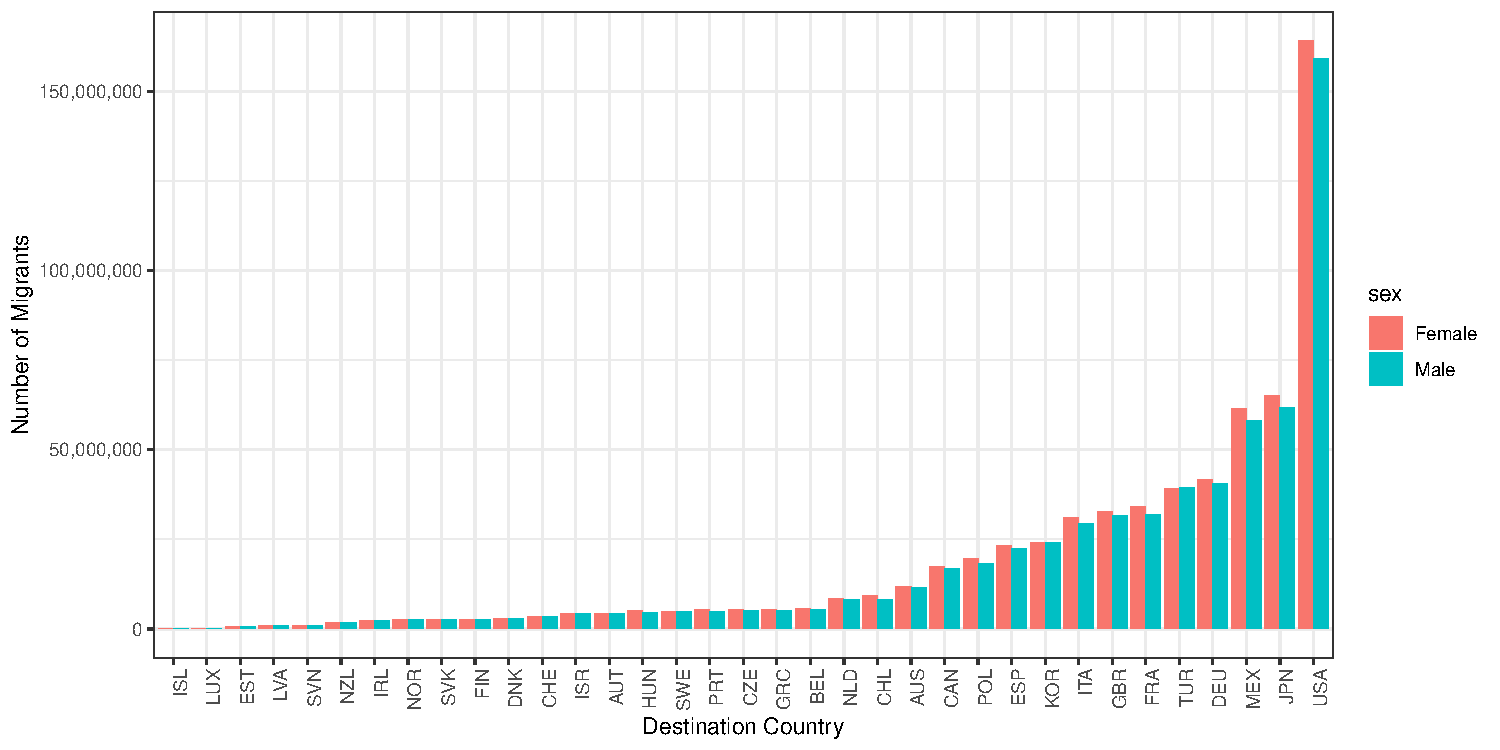
\includegraphics{ETC5513assignment4_files/figure-latex/gendergap-1.pdf}
\caption{\label{fig:gendergap}Gender difference in migrant population in countries}
\end{figure}

In 2015-16, the most number of migrants fell in the age group 25-64, with females being higher in number compared to males in countries like the USA, Mexico, Germany, etc. In countries like Japan, Korea and Spain it can be seen that there is no gender gap in the migrant population of age group 25-64 whereas in countries like Poland and Turkey the number of males is higher than females for the same age group.
Amongst the age group 15-24, there is a relatively low gender difference in the migrant population compared to the other age groups and the trend is uniform in almost all the countries whereas amongst the migrants who are 65 years old and above, the number of females is higher than that of males in the USA, Japan , Italy, etc and Mexico being one of the top destinations for migration, saw an influx of an equal number of males and females aged over 65 in the year 2015-16.

\begin{figure}
\centering
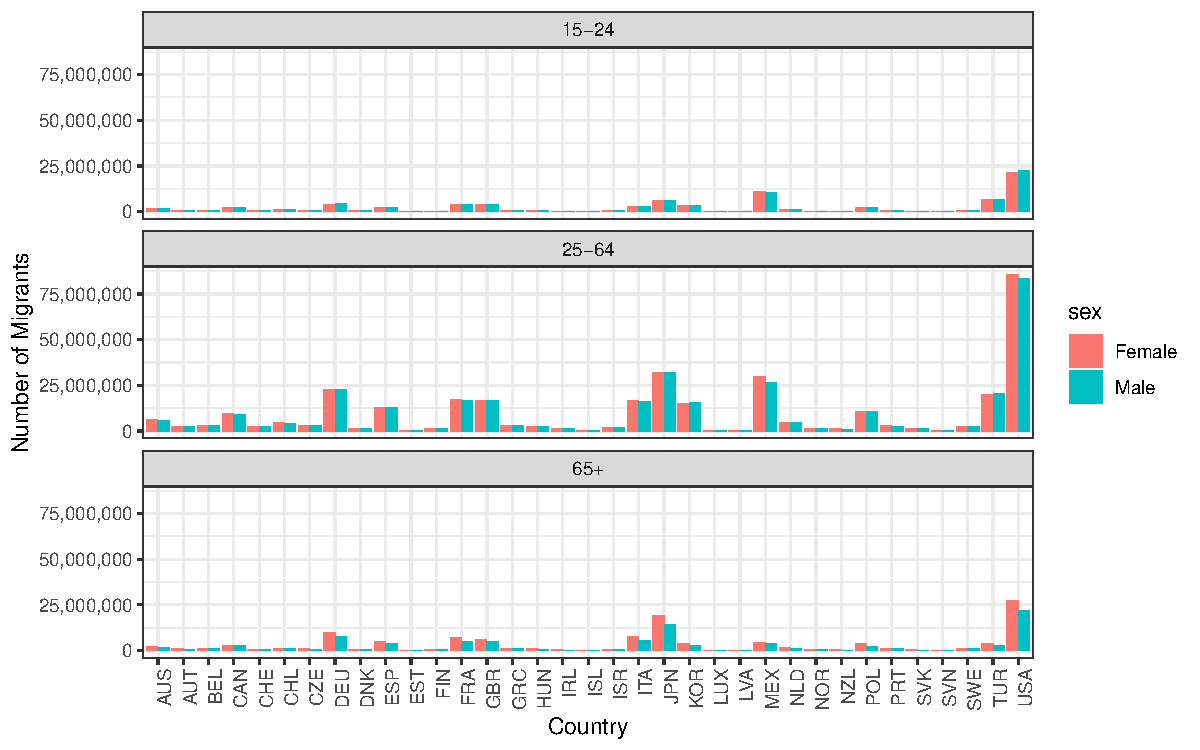
\includegraphics{ETC5513assignment4_files/figure-latex/agegap-1.pdf}
\caption{\label{fig:agegap}Gender difference in migrant population across age groups in countries}
\end{figure}

\section*{Limitations}

The Database on Immigrants in OECD Countries (DIOC) 2015/16 provides information on age,duration of stay, labour force status and occupation of the migrants. The limitations of the dataset is as follows,

\begin{enumerate}

   \item Confidentiality and Reliability issues 

Due to confidentiality issues, the place of birth is recorded at the continental level such as Africa, Asia, Europe, etc.instead of the country level in the dataset,therefore the analysis is focused on only the destination countries.Also,there is only limited details available on the important variables like educational qualification and skills. 

   \item Unavailability of data

Unavailability of data on variables like age, skills,occupation ,labour force status and educational qualification proved to be a limitation to the analysis of the dataset.

 \item  Inconsistency of data
 
 The dataset contains inconsistency in data for example the reference population for Switzerland, Luxembourg and New Zealand is 15+ and there is no information on the age group 0-14. Due to this reason and the fact that 0-14 age group belongs to the minor category, the age group 0-14  was not considered for the analysis of gender gap in migrant population.  
 
 \end{enumerate}

\section*{Conclusion}

Migrants have made significant impacts on socio-economic as well as the political sphere of a destination countries. From the analysis on the Database on Immigrants in OECD Countries (DIOC) released by The Organisation for Economic Co-operation and Development (OECD), we conclude the following,

\begin{enumerate}

\item In the year 2015-16 , 50.94 % of international migrants were female where as 49.06% were male. 

\item People between 25-64 years old migrated more compared to the other age groups in year 2015-16. 


\end{enumerate}

\nocite{*}

\printbibliography

\end{document}

